\documentclass[border=8pt]{standalone}
\usepackage[T1]{fontenc}\usepackage{helvet}\renewcommand{\familydefault}{\sfdefault}
\usepackage{tikz}\usetikzlibrary{shapes.geometric, arrows.meta, positioning, calc, backgrounds}
\definecolor{ink}{HTML}{1a1916}
\definecolor{inktwo}{HTML}{3a3a35}
\definecolor{inkthree}{HTML}{6a6862}
\definecolor{rule}{HTML}{b8b09a}
\definecolor{amber}{HTML}{a8730a}
\definecolor{red}{HTML}{c8261a}
\definecolor{paper}{HTML}{f0eee5}
\definecolor{slab}{HTML}{d8d4c6}
\definecolor{ghost}{HTML}{cfc9b6}
\tikzset{
  >={Stealth[length=2.4mm]},
  wire/.style={line width=0.7pt, ink},
  modwire/.style={line width=0.6pt, dashed, ink},
  tastewire/.style={line width=0.6pt, dashed, amber},
  block/.style={rectangle, draw=ink, line width=0.9pt, fill=slab, minimum width=20mm, minimum height=10mm, inner sep=2pt, align=center, font=\footnotesize\bfseries, text=ink},
  ghost/.style={rectangle, draw=ghost, line width=0.6pt, dashed, minimum width=20mm, minimum height=10mm, inner sep=2pt, align=center, font=\footnotesize, text=ghost},
  perf/.style={rectangle, draw=ink, line width=0.7pt, minimum width=20mm, minimum height=7mm, inner sep=2pt, font=\footnotesize, text=ink},
  perfghost/.style={perf, draw=ghost, text=ghost, dashed, line width=0.5pt},
  ess/.style={font=\scriptsize, text=ink, align=left, anchor=north west, inner sep=1pt, text width=2.3cm},
  tst/.style={font=\scriptsize, text=amber, align=left, anchor=north west, inner sep=1pt, text width=2.3cm},
  tap/.style={circle, fill=ink, minimum size=3.4pt, inner sep=0pt},
}
\begin{document}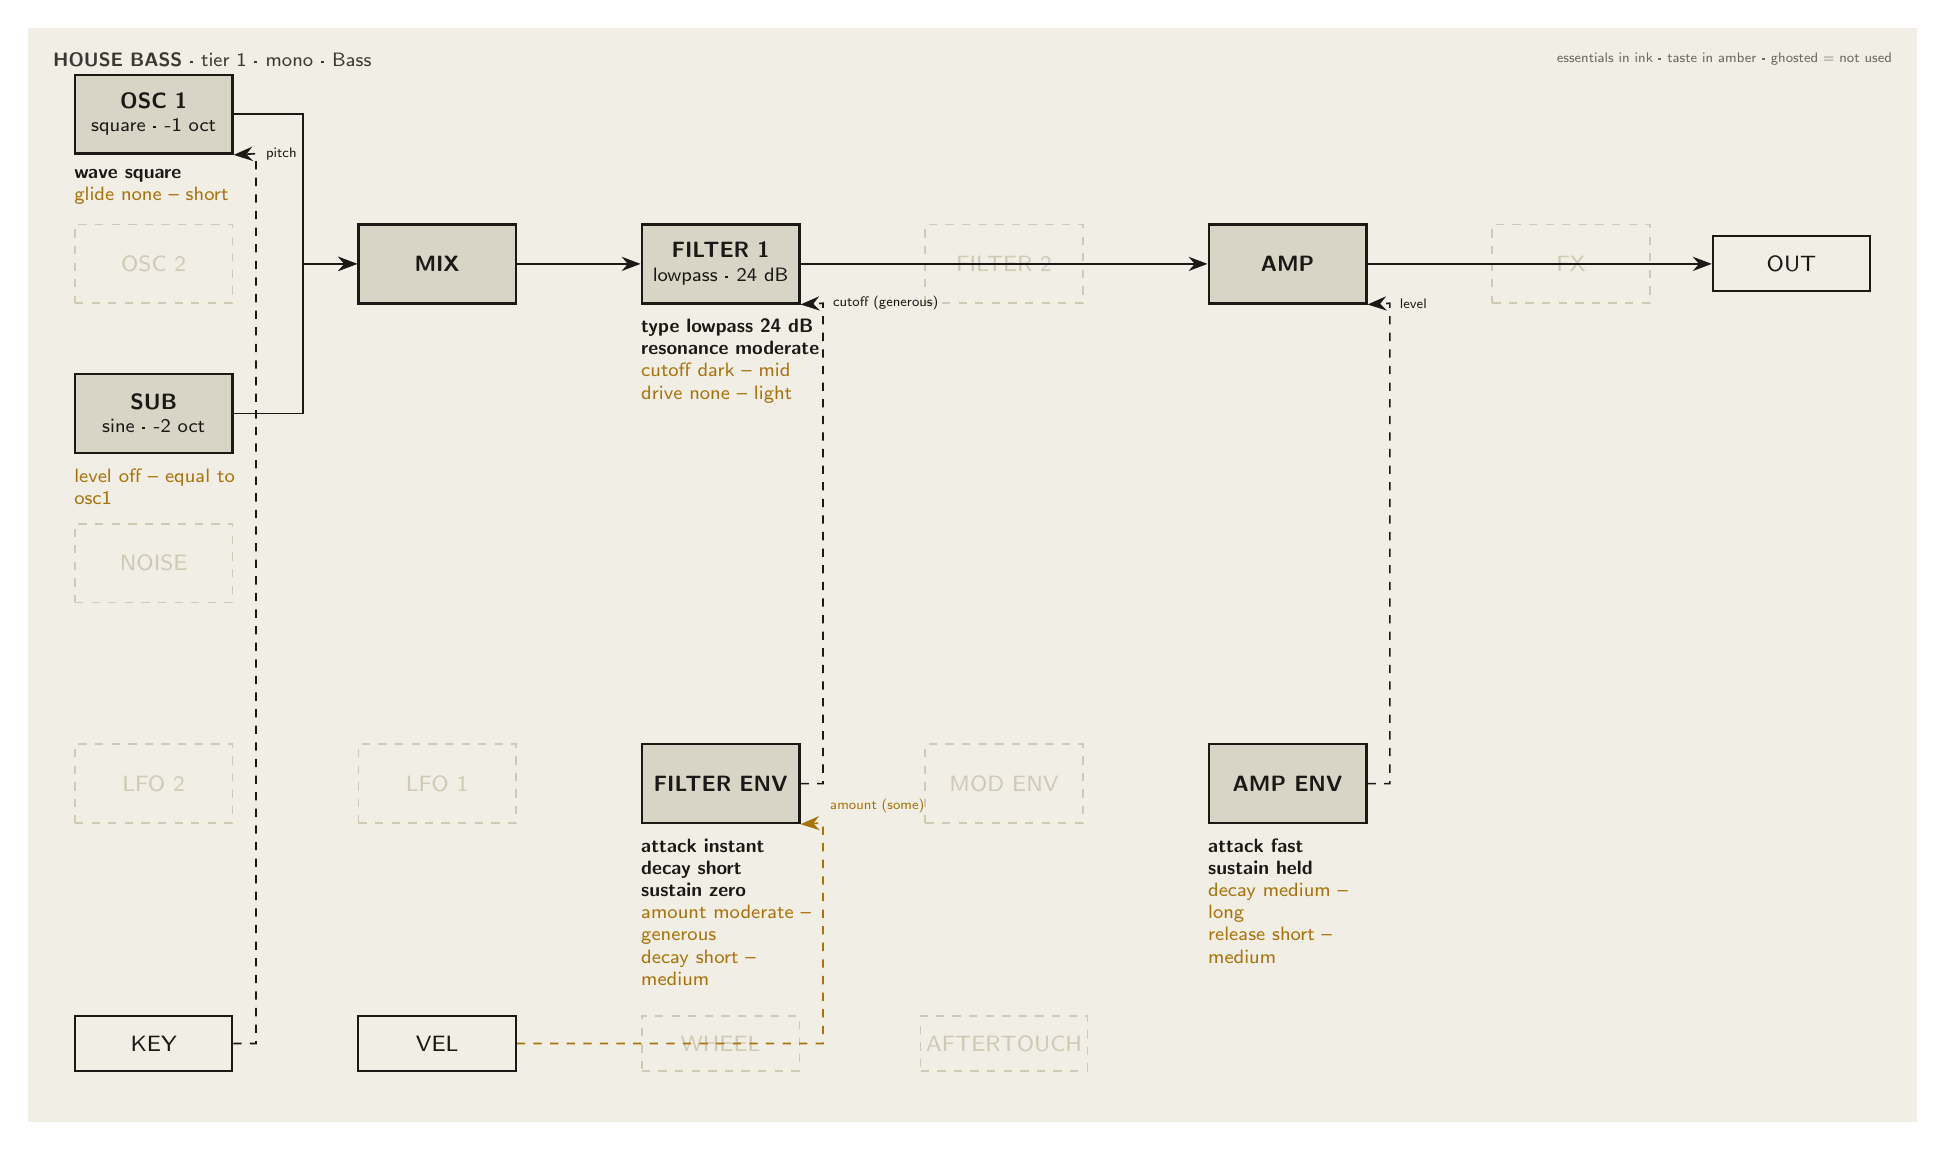
\begin{tikzpicture}
\begin{scope}[on background layer]\fill[paper] (-1.6,-10.9) rectangle (22.4,3.0);\end{scope}
\node[block] (osc1) at (0.0,1.9) {OSC 1\\[-1pt]{\scriptsize\mdseries square · -1 oct}};
\node[ess] at (-1.05,1.2399999999999998) {\textbf{wave square} \\ \textcolor{amber}{glide none -- short}};
\node[ghost] (osc2) at (0.0,0.0) {OSC 2};
\node[block] (sub) at (0.0,-1.9) {SUB\\[-1pt]{\scriptsize\mdseries sine · -2 oct}};
\node[ess] at (-1.05,-2.56) {\textcolor{amber}{level off -- equal to osc1}};
\node[ghost] (noise) at (0.0,-3.8) {NOISE};
\node[block] (mix) at (3.6,0.0) {MIX};
\node[block] (filter1) at (7.2,0.0) {FILTER 1\\[-1pt]{\scriptsize\mdseries lowpass · 24 dB}};
\node[ess] at (6.15,-0.66) {\textbf{type lowpass 24 dB} \\ \textbf{resonance moderate} \\ \textcolor{amber}{cutoff dark -- mid} \\ \textcolor{amber}{drive none -- light}};
\node[ghost] (filter2) at (10.8,0.0) {FILTER 2};
\node[block] (amp) at (14.4,0.0) {AMP};
\node[ghost] (fx) at (18.0,0.0) {FX};
\node[ghost] (lfo2) at (0.0,-6.6) {LFO 2};
\node[ghost] (lfo1) at (3.6,-6.6) {LFO 1};
\node[block] (fenv) at (7.2,-6.6) {FILTER ENV};
\node[ess] at (6.15,-7.26) {\textbf{attack instant} \\ \textbf{decay short} \\ \textbf{sustain zero} \\ \textcolor{amber}{amount moderate -- generous} \\ \textcolor{amber}{decay short -- medium}};
\node[ghost] (menv) at (10.8,-6.6) {MOD ENV};
\node[block] (aenv) at (14.4,-6.6) {AMP ENV};
\node[ess] at (13.35,-7.26) {\textbf{attack fast} \\ \textbf{sustain held} \\ \textcolor{amber}{decay medium -- long} \\ \textcolor{amber}{release short -- medium}};
\node[perf] (key) at (0.0,-9.9) {KEY};
\node[perf] (vel) at (3.6,-9.9) {VEL};
\node[perfghost] (wheel) at (7.2,-9.9) {WHEEL};
\node[perfghost] (at) at (10.8,-9.9) {AFTERTOUCH};
\node[perf, draw=ink, fill=paper] (out) at (20.8,0.0) {OUT};
\draw[wire,->] (osc1.east) -- (1.9,1.9) |- (mix.west);
\draw[wire,->] (sub.east) -- (1.9,-1.9) |- (mix.west);
\draw[wire,->] (mix.east) -- (filter1.west);
\draw[wire,->] (filter1.east) -- (amp.west);
\draw[wire,->] (amp.east) -- (out.west);
\draw[modwire,->] (fenv.east) -- (8.5,-6.6) -- (8.5,-0.5) node[pos=1, right, font=\tiny, text=ink] {cutoff (generous)} -- (filter1.south east);
\draw[modwire,->] (aenv.east) -- (15.700000000000001,-6.6) -- (15.700000000000001,-0.5) node[pos=1, right, font=\tiny, text=ink] {level} -- (amp.south east);
\draw[modwire,->] (key.east) -- (1.3,-9.9) -- (1.3,1.4) node[pos=1, right, font=\tiny, text=ink] {pitch} -- (osc1.south east);
\draw[tastewire,->] (vel.east) -- (4.9,-9.9) -- (8.5,-9.9) -- (8.5,-7.1) node[pos=1, above right, font=\tiny, text=amber, xshift=-1pt] {amount (some)} -- (fenv.south east);
\node[anchor=north west, font=\scriptsize, text=inktwo] at (-1.4,2.8) {\textbf{HOUSE BASS} · tier 1 · mono · Bass};
\node[anchor=north east, font=\tiny, text=inkthree] at (22.2,2.8) {essentials in ink · taste in amber · ghosted = not used};
\end{tikzpicture}\end{document}
